\section{The LLaMA 3 Herd of Models}
\begin{frame}{}
    \LARGE \textbf{The LLaMA 3 Herd of Models}
\end{frame}

\begin{frame}[allowframebreaks]{The LLaMA 3 Herd of Models}
    \begin{figure}
        \centering
        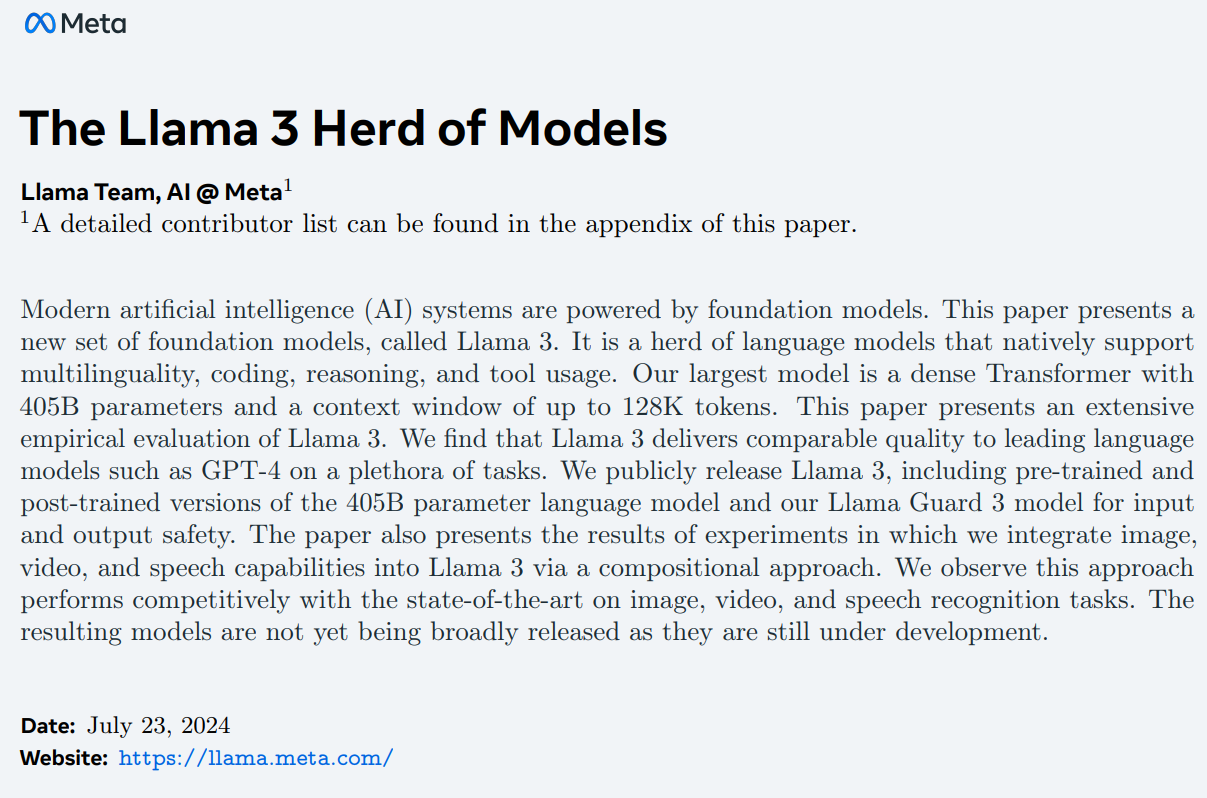
\includegraphics[height=0.80\textheight,width=\textwidth,keepaspectratio]{images/recent-advance/llama-3-paper.png}
        \caption*{\scriptsize Source: Llama Team, AI @ Meta, ``The Llama 3 Herd of Models,'' \href{https://arxiv.org/abs/2407.21783}{arXiv:2407.21783}, title page.}
    \end{figure}
\framebreak
    \textbf{Meta AI (2024)}

    \begin{itemize}
        \item \textbf{Model Sizes:} 8B, 70B, and 405B
        \item \textbf{Open Weights:} Available for commercial use
        \item \textbf{Training:} The 405B model is pre-trained on 15.6 trillion multilingual tokens, against 1.8 trillion for LLaMA 2
        \item \textbf{Architecture:} A standard dense transformer; the gains come from data quality and training scale rather than architectural novelty
    \end{itemize}

\framebreak

    \begin{figure}
        \centering
        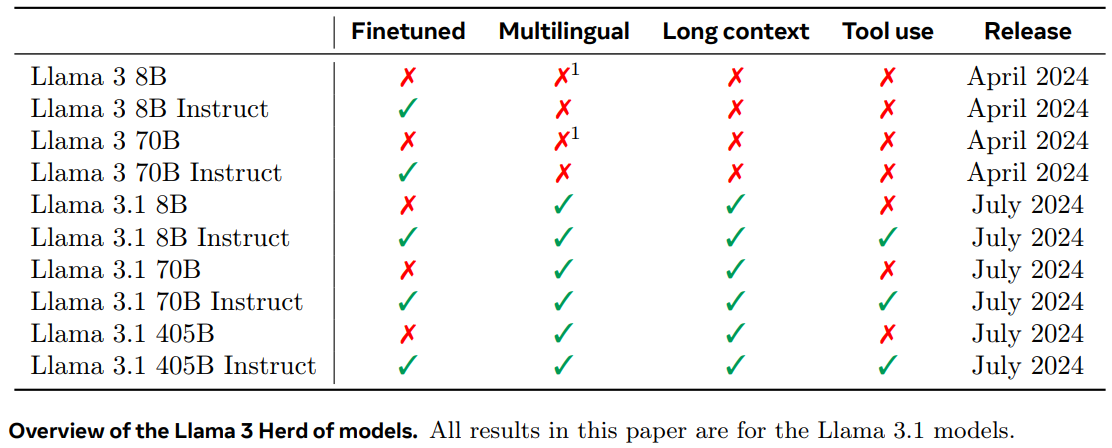
\includegraphics[height=0.76\textheight,width=\textwidth,keepaspectratio]{images/recent-advance/llama-3-models.png}
        \caption*{\scriptsize The April 2024 release (8B, 70B) is short-context and was intended for English use at the time; the multilingual, long-context, tool-using models arrive with LLaMA 3.1 in July 2024, and every result in the paper is for those. Source: Llama Team, AI @ Meta, \href{https://arxiv.org/abs/2407.21783}{arXiv:2407.21783}, Table~1.}
    \end{figure}

\framebreak

    \textbf{Key Features:}
    \begin{itemize}
        \item Context window of up to 128k tokens, reached in two stages: pre-training at 8k, then continued pre-training on longer sequences
        \item Grouped-query attention with 8 key-value heads, which shrinks the key-value cache and speeds up decoding
        \item A 128k-token vocabulary: 100k from the \texttt{tiktoken} tokenizer plus 28k added for non-English languages
        \item FP8 quantization of the feed-forward layers for low-precision inference on H100 GPUs; the self-attention layers are left unquantized
        \item Released fine-tuned variants are the Instruct models
    \end{itemize}

\framebreak

    \begin{figure}
        \centering
        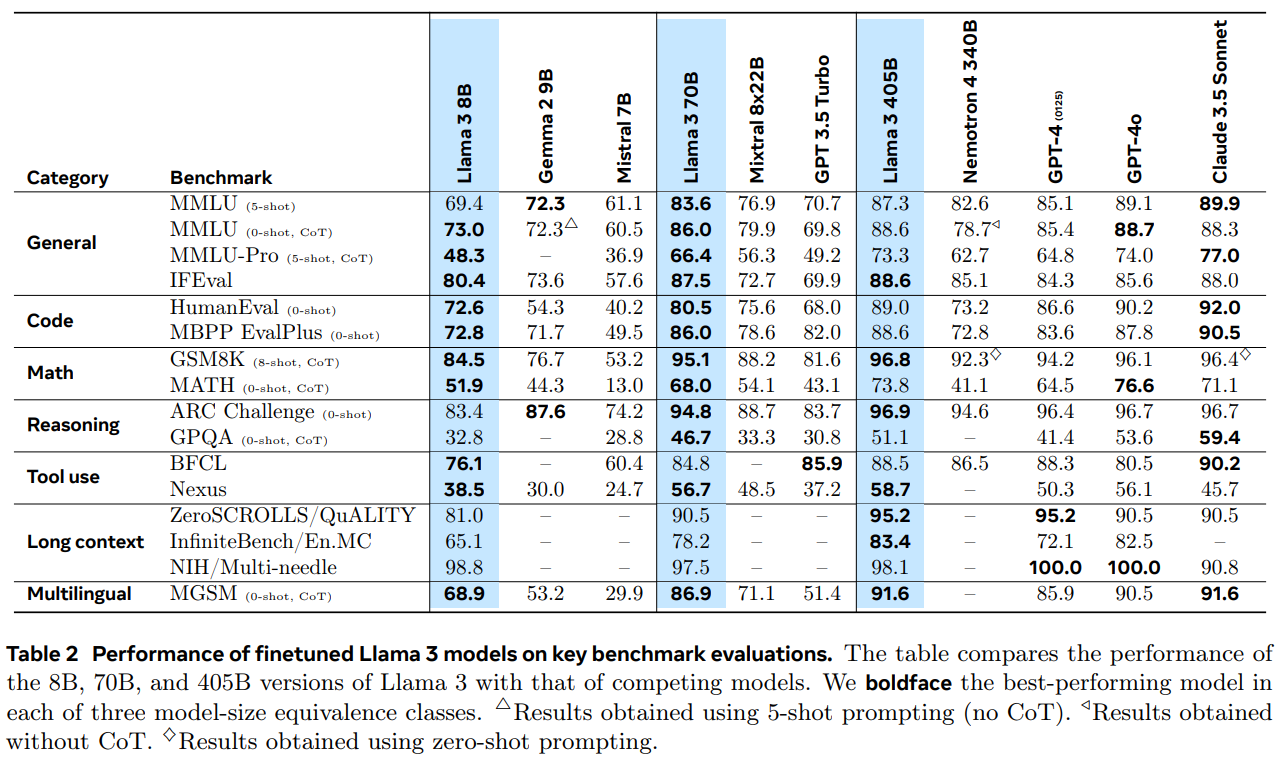
\includegraphics[height=0.78\textheight,width=\textwidth,keepaspectratio]{images/recent-advance/llama-3-performance.png}
        \caption*{\scriptsize Source: Llama Team, AI @ Meta, \href{https://arxiv.org/abs/2407.21783}{arXiv:2407.21783}, Table~2.}
    \end{figure}

\framebreak

    \begin{figure}
        \centering
        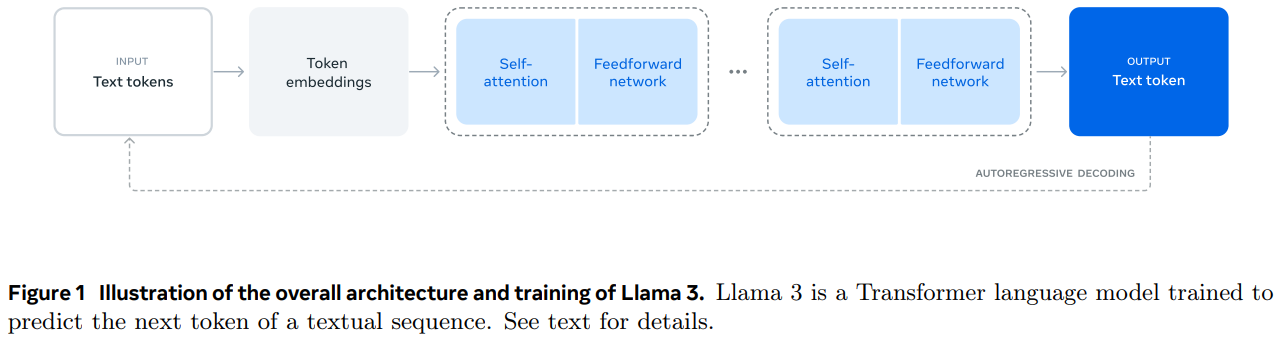
\includegraphics[height=0.72\textheight,width=\textwidth,keepaspectratio]{images/recent-advance/llama-3-architecture.png}
        \caption*{\scriptsize Source: Llama Team, AI @ Meta, \href{https://arxiv.org/abs/2407.21783}{arXiv:2407.21783}, Figure~1.}
    \end{figure}

\framebreak

    \begin{figure}
        \centering
        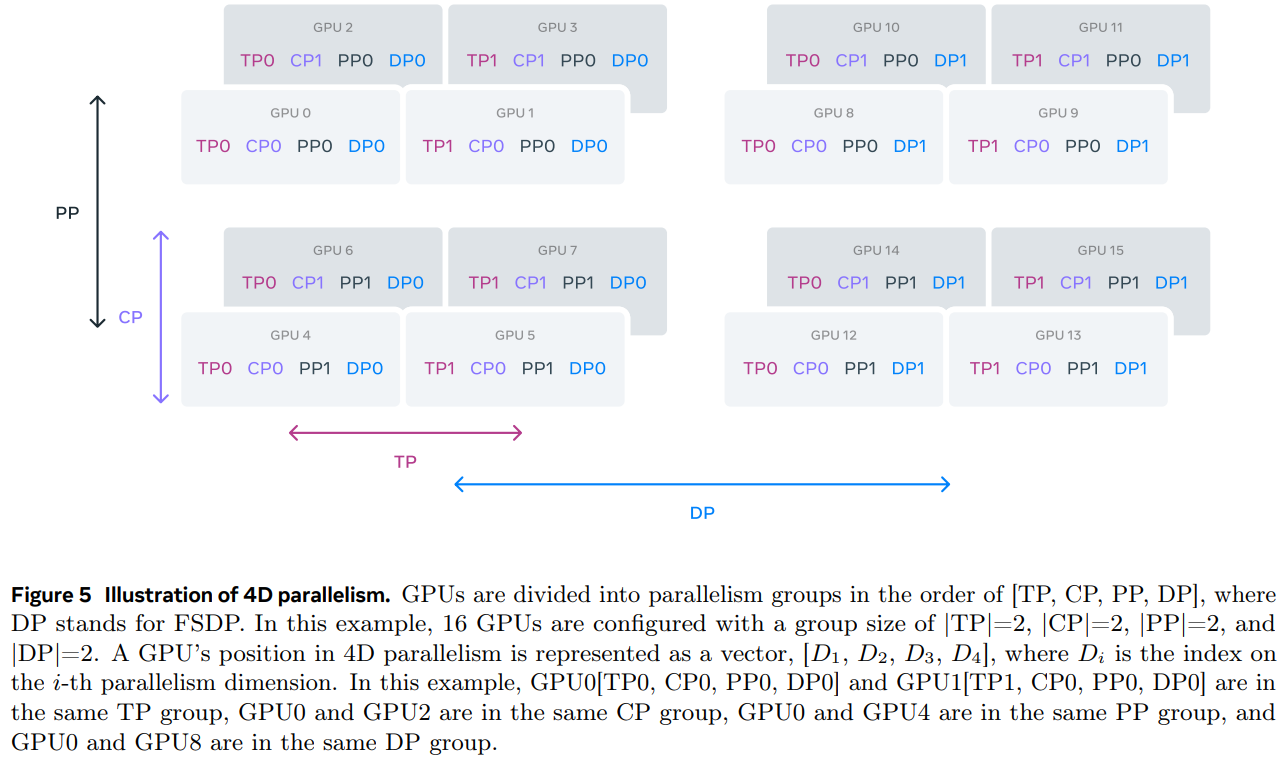
\includegraphics[height=0.76\textheight,width=\textwidth,keepaspectratio]{images/recent-advance/llama-3-4d-parallel.png}
        \caption*{\scriptsize Training the 405B model splits each batch across four parallelism dimensions at once: tensor, context, pipeline, and data. Source: Llama Team, AI @ Meta, \href{https://arxiv.org/abs/2407.21783}{arXiv:2407.21783}, Figure~5.}
    \end{figure}

\framebreak

    \begin{figure}
        \centering
        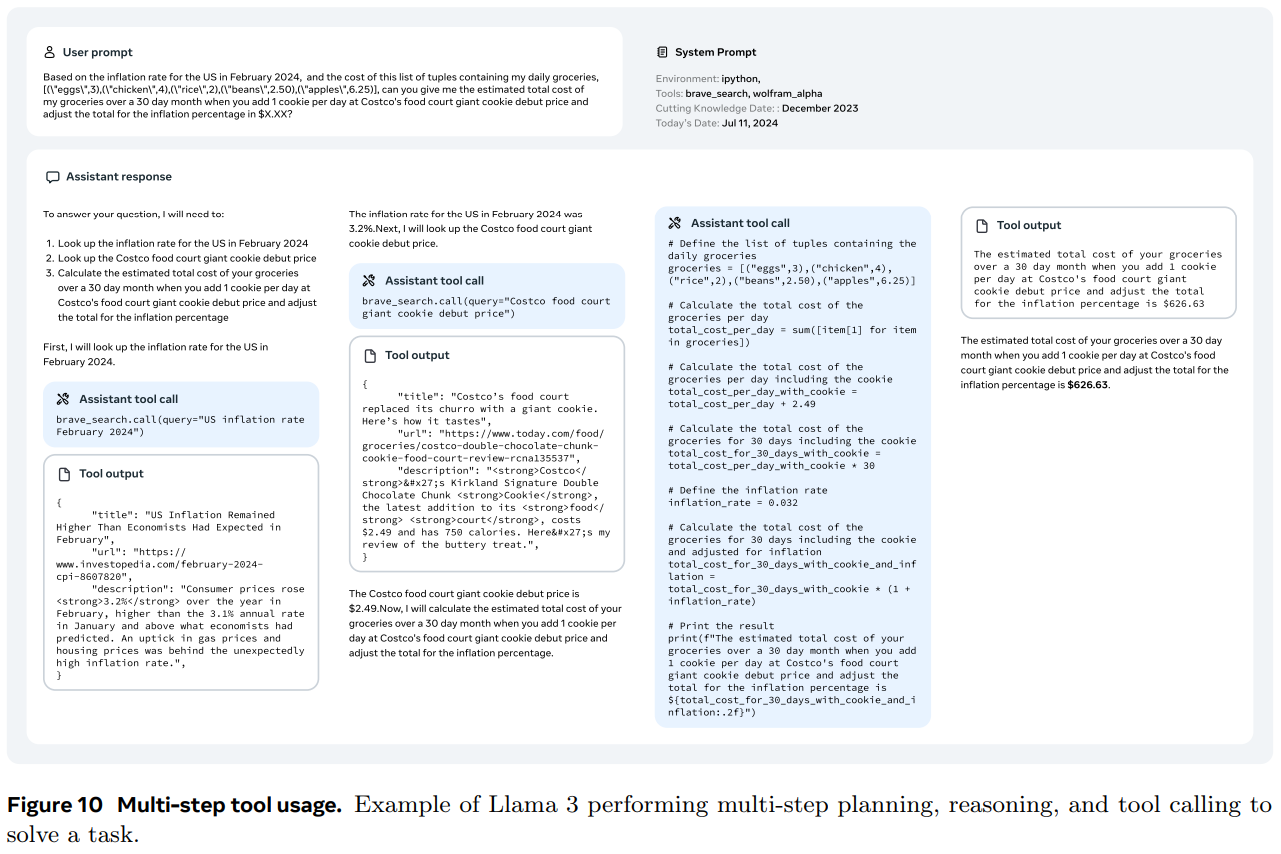
\includegraphics[height=0.80\textheight,width=\textwidth,keepaspectratio]{images/recent-advance/llama-3-example.png}
        \caption*{\scriptsize Source: Llama Team, AI @ Meta, \href{https://arxiv.org/abs/2407.21783}{arXiv:2407.21783}, Figure~10.}
    \end{figure}

\framebreak

    \begin{figure}
        \centering
        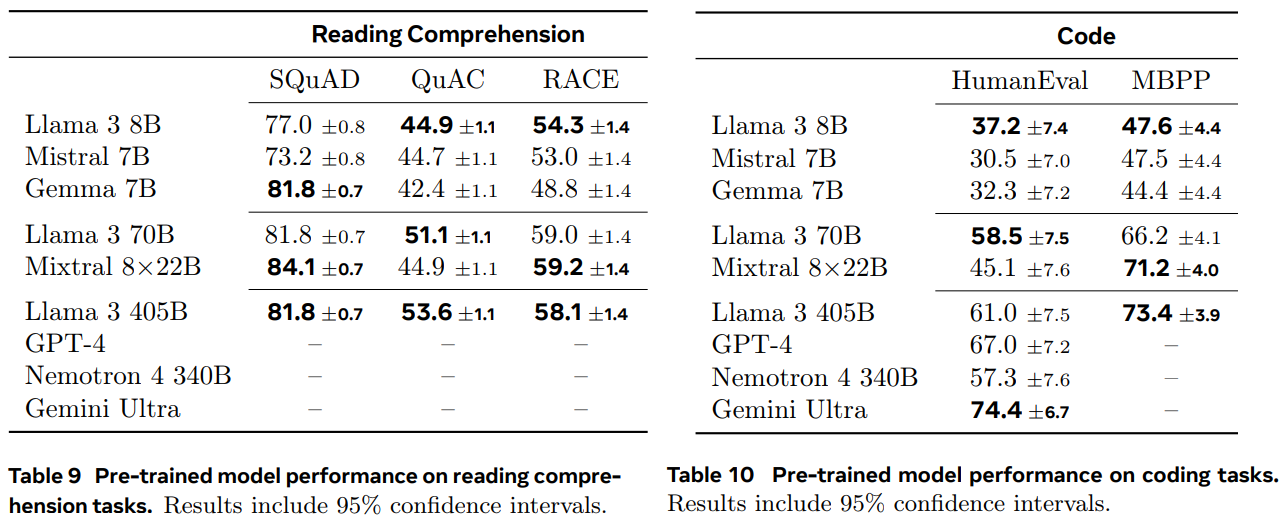
\includegraphics[height=0.78\textheight,width=\textwidth,keepaspectratio]{images/recent-advance/llama-3-compare.png}
        \caption*{\scriptsize Source: Llama Team, AI @ Meta, \href{https://arxiv.org/abs/2407.21783}{arXiv:2407.21783}, Tables~9 and~10.}
    \end{figure}

\framebreak

    \textbf{Highlights:}
    \begin{itemize}
        \item Quality comparable to leading closed models such as GPT-4 across a broad benchmark suite
        \item Image, video, and speech capabilities are added compositionally: adapters and cross-attention layers are trained on top of the language model while its weights stay frozen, so text-only quality is preserved
        \item Those multimodal variants were still under development, and not released, at publication
    \end{itemize}
\end{frame}
